\documentclass[a4paper,fleqn,usenatbib]{mnras}
\pdfoutput=1
% MNRAS is set in Times font. If you don't have this installed (most LaTeX
% installations will be fine) or prefer the old Computer Modern fonts, comment
% out the following line
%\usepackage{newtxtext,newtxmath}
% Depending on your LaTeX fonts installation, you might get better results with one of these:
%\usepackage{mathptmx}
%\usepackage{txfonts}

% Use vector fonts, so it zooms properly in on-screen viewing software
% Don't change these lines unless you know what you are doing
\usepackage[T1]{fontenc}
\usepackage{ae,aecompl}
\usepackage{epstopdf}
\usepackage{aas_macros}
\usepackage{braket}
\usepackage{verbatim}
\usepackage{wrapfig}
\usepackage{booktabs}
\usepackage{amsfonts}
\usepackage{amsmath}
\usepackage{appendix}
\usepackage{graphicx}
\usepackage[usenames,dvipsnames]{color}
\usepackage[normalem]{ulem}
\usepackage{array}
\bibliographystyle{mnras}


\newcommand{\myemail}{samuelreay@gmail.com}
\newcommand{\tick}{\checkmark}
\newcommand{\gtick}{\color{ForestGreen} \tick }
\newcommand{\cross}{$\times$ }
\newcommand{\rcross}{\color{red} \cross }
\newcommand{\runz}{\textsc{Runz}}
\newcommand{\brac}[1]{\left( #1 \right)}
\newcommand*\mean[1]{\bar{#1}}
\newcommand\abs[1]{\left|#1\right|}
\newcommand {\etal} {\emph{~et~al.} }
\newcommand{\green}{\color{green}}
\newcommand{\blue}{\color{blue}}
\newcommand{\red}{\color{red}}
\newcommand{\orange}{\color{BurntOrange}}
\newcommand{\purple}{\color{Fuchsia}}
\newcommand{\hMpc}{h^{-1} {\rm Mpc}} % to be used in math mode
\newcommand{\camb}{\textsc{camb}}
\newcommand{\cosmomc}{\textsc{cosmomc}}

\newcommand{\kmsmpc}{km\,s$^{-1}$\,Mpc$^{-1}$}

\newcommand{\halofit}{\textsc{halofit}}
\newcommand{\specialcell}[2][c]{\begin{tabular}[#1]{@{}c@{}}#2\end{tabular}}



%\shortauthors{}
\title[Correcting for sample selection in Bayesian analyses]{Correcting for sample selection in Bayesian analyses}

\author[S. R. Hinton et al.]{Samuel R. Hinton,$^{1,2}$\thanks{E-mail: \href{samuelreay@gmail.com}}
	Alex Kim,$^{3}$
	Tamara M. Davis,$^{1,2}$
\\
% List of institutions
$^{1}$School of Mathematics and Physics, The University of Queensland, Brisbane, QLD 4072, Australia\\
$^{2}$ARC Centre of Excellence for All-sky Astrophysics (CAASTRO)\\
$^{3}$Lawrence Berkeley National Labs
}
% These dates will be filled out by the publisher
\date{Accepted XXX. Received YYY; in original form ZZZ}

% Enter the current year, for the copyright statements etc.
\pubyear{2017}

\begin{document}


\label{firstpage}
\pagerange{\pageref{firstpage}--\pageref{lastpage}}
\maketitle





\begin{abstract}
Lifetimes are strictly positive. We cut our data to remove background noise.  Astronomical observations suffer from Malmquist bias - our samples are preferentially biased toward those sources that are more likely to be observationally detected. These sample selections should be accounted for. In this paper we present a simple overview of a Bayesian consideration of sample selection, giving a solution to both analytically tractable and intractable models. This can be accomplished via a combination of analytic approximations and Monte Carlo integration, in which dataset simulation is efficiently used to correct for issues in the observed dataset. Toy models are included, along with numerical considerations and optimisations for implementation.
\end{abstract}








\section{Introduction}

Sample selection is a problem in many areas of scientific inquiry. It is one of the primary difficulties when performing supernovae cosmology analysis, as our telescopes have visual limits that modify our observed supernovae distribution from the actual underlying distribution. This bias, termed Malmquist bias, is source of much investigation \citep{Butkevich2005}. It is considered during analysis by either modifying the observed data to remove the expected bias \citep{BetouleKessler2014, ConleyGuySullivan2011}, or by incorporating the expected bias into the underlying model \citep{Rubin2015}. Truncated data is also commonly encountered in biological fields, where data such as mortality rates are left-truncated \citep{JANE1898}. Simplified and generalised examples have been investigated in numerous fashions \citep{woodroofe1985estimating, Gull1989bayesian, grogger1991models, o1995truncated} and with different fitting algorithms \citep{Gelfand1992}. Whilst generalised resources exist that provide a comprehensive overview of sample selection and analysis techniques in a similar fashion to this work \citep{klein2005survival}, these sources are often opaque due to volume and mathematical complexity. 

This work provides a simple treatment of sample selection in a common Bayesian technique. The general theory for considering selection effects is discussed in Section \ref{sec:theory}. Section \ref{sec:examples} provides three examples of increasing complexity with sample selection. Section \ref{sec:tricks} details numeric concerns and tricks to be aware of for effective implementation of Monte Carlo corrections applied to analytic approximations.






\section{Theory}
\label{sec:theory}

When formulating and fitting a model using a constraining dataset, we wish to resolve the posterior surface defined by
\begin{align}
P(\theta | {\rm data}) \propto P({\rm data} | \theta) P(\theta).
\end{align}
Of primary interest to us is the likelihood of observing the data given our parametrised model, $\mathcal{L} \equiv P({\rm data} | \theta)$. When dealing with experiments which have selection efficiency, our likelihood necessarily includes that efficiency, for we want to describe the probability that our observations were both drawn from the underlying theoretical model \textit{and} that those observations, given they happened, were subsequently successfully observed.  To make this extra conditional explicit, we can write our likelihood as
with selection effect $S$:
\begin{align}
\mathcal{L} &= P({\rm data} | \theta, S). \label{eq:like}
\end{align}
As we wish to describe our selection efficiency generally as a function dependent on both our data and our model, we can reformulate to
\begin{align}
\mathcal{L}&= \frac{P(S|{\rm data},\theta) P({\rm data}|\theta)}{P(S|\theta)}.
\end{align}
Introducing an integral over all possible data to make $P(S|\theta)$ physical,
\begin{align}
\mathcal{L}&= \frac{P(S|{\rm data},\theta) P({\rm data}|\theta)}{\int P(S, D|\theta)\, dD} \\
&= \frac{P(S|{\rm data},\theta) P({\rm data}|\theta)}{\int P(S | D, \theta) P(D|\theta)\, dD}, \label{eq:main}
\end{align}
where the integral in the denominator has the same dimensionality is the experimental data. \textbf{Equation \ref{eq:main} is the generalised likelihood of experiments with sample selection.}




\section{Sample Selection}
\label{sec:examples}

 In this section we present sample selections of increasing complexity. Each sample selection is accompanied by an illustrative example inspired by Type Ia supernova cosmology, where we characterize the properties of a standard or standardizable candle.
 
 
\subsection{Complete Selection}
\label{sec:perfect}
In a perfect world, data is neither biased nor truncated. The data is perfect. Uncertainties are well quantified and normally distributed around true values. Presumably everything is also spherical and in a vacuum. We thus begin by considering an ideal situation where the sample is complete.  All events are included in the sample such that per object, $P(S | {\rm data}, \theta)=1$.  Trivially this expression is independent of $\theta$, and our likelihood from equation \eqref{eq:main} reduces down to equation \eqref{eq:like}. As a concrete example of this case, let us consider a model for a population of objects whose brightnesses form a normal distribution with average $\mu$ and standard deviation $\sigma$.
Let us also assume that our experiment produces data $x$, measurements of the brightnesses with negligible measurement uncertainty, which we can formally state as
\begin{align}
\vec{x} \sim \mathcal{N}(\mu,\sigma).
\end{align}
If, having collected our observations $\vec{x}$, we wanted to constrain $\mu$ and $\sigma$, this would be a simple task of modelling the posterior surface. Taking uniform priors on both parameters, we simply wish to map the surface
\begin{align}
P(\theta | {\rm data}) \propto P({\rm data} | \theta) P(\theta),
\end{align}
where our model parameters $\theta = \lbrace \mu, \sigma \rbrace$ and our data is given by $\vec{x}$.
\begin{align}
P(\mu,\sigma| \vec{x}) &\propto P(\vec{x} | \mu, \sigma) P(\mu, \sigma)
\end{align}
With uniform priors, $P(\mu,\sigma) = {\rm constant}$, and can be absorbed into the constant of proportionality. Expanding our observation vector, the posterior surface is given by
\begin{align}
P(\mu,\sigma| \vec{x}) &\propto \prod_{i=1}^N \mathcal{N}(x_i | \mu, \sigma). \label{eq:prod}
\end{align}
Generating a hundred data points with $\mu=100,\ \sigma=10$, we can recover our input parameters easily, as shown in Figure \ref{fig:perfect}.
\begin{figure}
	\begin{center}
		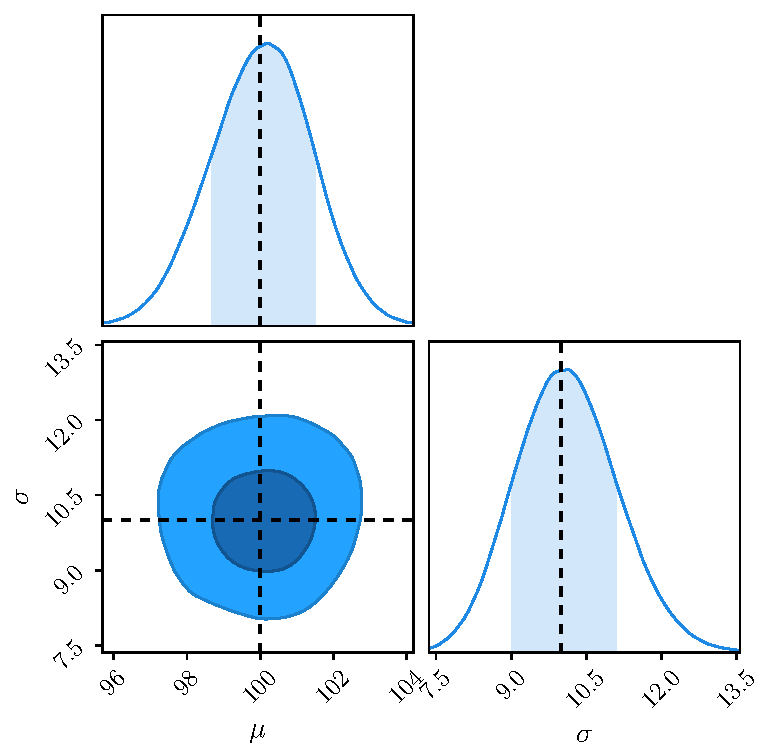
\includegraphics[width=\columnwidth]{example/perfect.pdf}
	\end{center}
	\caption{A systematic test of our perfect model, done by stacking the output chains from fitting 100 independent realisations of our 100 data points. Any systematic offset in our model would be revealed by a shift in the stacked results away from the true parameter values.}
	\label{fig:perfect}
\end{figure}










\subsection{Analytic Sample Selection}
\label{sec:imperfect}

We now consider a case with selection bias and has an analytic expression for the likelihood.  This illustrative case is useful for the reader as the influence of selection bias is simple and intuitive. The case we consider is identical to the one in the previous section, \textit{except} that only the subset of objects brighter than a threshold $\alpha$ can be observed.

With this sample selection, all events satisfy $x > \alpha$, giving $P(S|x,\theta) = \mathcal{H}(x - \alpha)$. We assign a value $\alpha=85$ for convenience. If we do not take this truncation into account, we will recover biased parameter estimates. However, we can correct for this truncation using equation \eqref{eq:main}, as the integral in the denominator has an analytic solution. Having successfully observed $x_i$, it follows that $x_i > \alpha$ and so $P(S|x_i,\theta) = 1$. To substitute in our normal model,
\begin{align}
\mathcal{L}_i &= \frac{P(S|x_i,\theta) P(x_i|\theta)}{\int P(S | D, \theta) P(D|\theta)\, dD} \\
&= \frac{ \mathcal{N}(x_i|\mu, \sigma)}{\int_{-\infty}^\infty \mathcal{H}(D - \alpha) \mathcal{N}(D|\mu, \sigma)\, dD} \\
&= \frac{ \mathcal{N}(x_i|\mu, \sigma)}{\int_{\alpha}^\infty \mathcal{N}(D|\mu, \sigma)\, dD} \\
&= \frac{ \mathcal{N}(x_i|\mu, \sigma)}{\frac{1}{2} {\rm erfc}\left[ \frac{\alpha - \mu}{\sqrt{2}\sigma} \right]}, 
\end{align}
where in the last line we have evaluated the integral in the case $\mu > \alpha$. Note that this is for a single observation, and so for a set of independent observations we need to introduce the product found in equation \eqref{eq:prod}. 
\begin{align}
\mathcal{L} &= \prod_{i=1}^N \mathcal{L}_i =  \prod_{i=1}^N \frac{ \mathcal{N}(x|\mu, \sigma)}{\frac{1}{2} {\rm erfc}\left[ \frac{\alpha - \mu}{\sqrt{2}\sigma} \right]}, 
\end{align}
However, as our selection efficiency correction is observationally independent it is identical for all observations, allowing us to take it outside the product.
\begin{align}
\mathcal{L} &= 2 \left( {\rm erfc}\left[ \frac{\alpha - \mu}{\sqrt{2}\sigma} \right] \right)^{-N}\prod_{i=1}^N  \mathcal{N}(x|\mu, \sigma), 
\end{align}
We can add this correction to our model, and note that we now recover unbiased parameter estimates. This is demonstrated in Figure \ref{fig:imperfect}, which shows the posterior surfaces for when you take sample selection into account and when you do not. The selection bias preferentially selects intrinsically brighter objects and, by cutting out some of the distribution, narrows the observed distribution, and so we note that the bias correction correctly increases the weight of low $\mu$ and high $\sigma$ parametrisations, as those models would be subject to the most sample bias. We also note that not only does the best fit location for each parameter shift, but the shape of the posterior surface itself is significantly modified.
\begin{figure}
	\begin{center}
		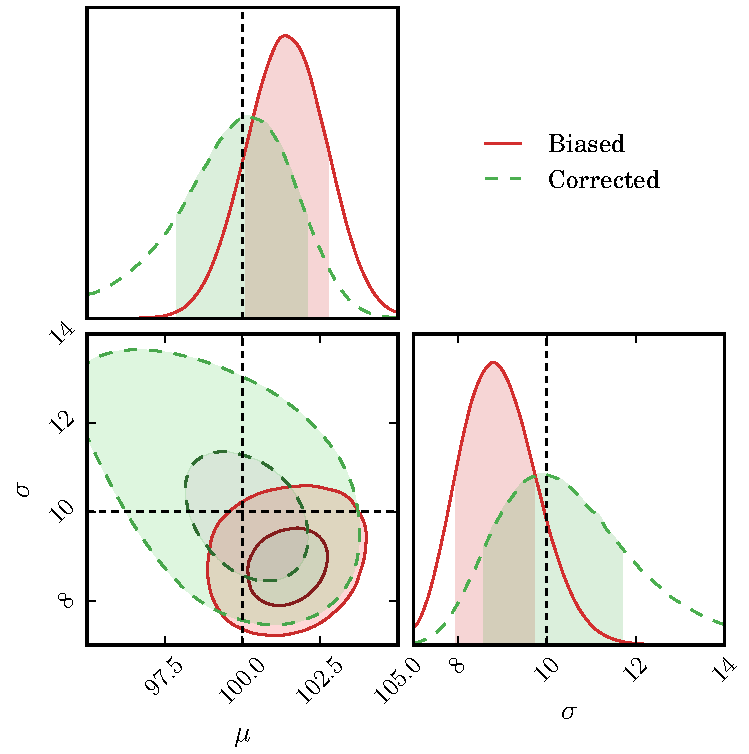
\includegraphics[width=\columnwidth]{example/imperfect.pdf}
	\end{center}
	\caption{A systematic test of our imperfect model, done by stacking the output chains from fitting 100 independent realisations of our 100 data points, subject to our thresholding. The bias shown in the red `Biased' contour can be corrected to via the techniques shown in Section \ref{sec:imperfect} to recover unbiased surfaces.}
	\label{fig:imperfect}
\end{figure}












\subsection{Analytically Intractable Sample Selection}
\label{sec:real}
Unfortunately it is a rare scenario when dealing with nature and all her faults for us to have an analytic selection function, let alone a function encapsulated by a single parameter. A more realistic scenario involves a selection efficiency instead would take the form of non-analytic function of many model parameters. And the function would probably be stochastic too, just to throw another wrench in the works. Provided a method of forward modelling or simulating observations, the solution is to combine an analytic approximate correction with Monte Carlo integration.

In this subsection we introduce an example that presents computational challenges in the evaluation of the posterior, and which better reflects the model complexity in supernova cosmology analysis. The specific challenge is that the denominator in the equation for the likelihood equation \eqref{eq:main} is dependent on $\theta$ and does not have an analytic solution (i.e. has to be solved numerically). When using Monte Carlo sampling methods to probe the posterior with this kind of likelihood, the integral in the denominator must be calculated with each draw. We therefore present importance sampling as an approach that make these posteriors more computationally tractable.

Let us modify our imperfect toy model from the previous section. Instead of observing just one variable, $x$, we also observe a new independent variable, $y$, which is drawn from its own distribution $y \sim \mathcal{N}(\mu_y, \sigma_y)$, and has no measurement uncertainty (like $x$). Our selection efficiency can now become a combination of $x$ and $y$, such that we only observe events that satisfy $x + \beta y > \alpha$, giving $P(S|x,y,\theta) = \mathcal{H}(x + \beta y - \alpha)$.  Our likelihood for such a toy model becomes now the combination of probabilities for observing both $x$ and $y$, with the denominator becoming an integral over all possible $X$ and $Y$ observations subject to our selection effects.
\begin{align}
\mathcal{L}_i &= \frac{ \mathcal{N}(x_i|\mu, \sigma) \mathcal{N}(y_i|\mu_y, \sigma_y)}
{\iint_{-\infty}^\infty \mathcal{H}(X + \beta Y - \alpha) \mathcal{N}(X|\mu, \sigma) \mathcal{N}(Y|\mu_y, \sigma_y)\, dX dY}
\end{align}
Assume that we cannot solve this integral analytically, and must resort to numeric solutions. These often clash with sampling methods, especially for high dimensional integrals. Inserting Monte Carlo integration into fitting algorithms can drastically slow them down, and algorithms such as Hamiltonian MCMC that require continuous surfaces can easily fail on surfaces that fluctuate from Monte Carlo integration. Even by fixing the samples used in MC integration (thereby giving a continuous surface), the complexity of the surface derivatives will pose almost insurmountable problems for any algorithms that utilise surface gradients.

One solution is to find an approximate, analytic correction we can utilise in our fitting algorithm which seeks to shift the region of parameter space sampled by the sampler closer to the correct area, and then importance sample our MC chains to provide a fully corrected surface. Given an approximate analytic correction $w_{\rm approx}$, we explicitly break our likelihood into two parts, $\mathcal{L}_i = \mathcal{L}_{i1} \mathcal{L}_{i2}$, with the parts given by
\begin{align}
\mathcal{L}_{i1} &= \frac{P(S|{\rm data},\theta) P({\rm data}|\theta)}{w_{\rm approx}} \\
\mathcal{L}_{i2} &= \frac{w_{\rm approx}}{\int P(S, D|\theta)\, dD}
\end{align}
Where $\mathcal{L}_{i1}$ represents an analytic function which can efficiently be sampled using traditional Monte Carlo sampling methods, and $\mathcal{L}_{i2}$ is a numerically calculated weight applied after Monte Carlo sampling in order to model the full likelihood surface.


In our example, if $\beta \ll 1$, such that the majority of selection effect is encapsulated by $x$ and not $y$, our approximate correction can take the form found in the previous correction from Section \ref{sec:imperfect}. Having true values of $\mu = 100$, $\sigma = 10$, $\mu_y = 30$, $\sigma_y = 5$, and a known $\beta = 0.2$, we can give a concrete example. Assuming some prior, imperfect knowledge of $\mu_y$ (perhaps we believe it is approximately $20$) we estimate that the average contribution from $\beta y$ is approximately $20\beta = 4$ (which is close to the correct value of $6$), and from this we add in a small adjustment to the analytic correction from Section \ref{sec:imperfect}:
\begin{align}
w_{\rm approx} = \frac{1}{2} {\rm erfc}\left[ \frac{\alpha - \mu - 4}{\sqrt{2}\sigma} \right].
\end{align}
This gives our likelihood parts as
\begin{align}
\mathcal{L}_{i1} &= \frac{ \mathcal{N}(x_i|\mu, \sigma) \mathcal{N}(y_i|\mu_y, \sigma_y)}{w_{\rm approx} } \\
\mathcal{L}_{i2} &= \frac{ w_{\rm approx}  }{\iint_{-\infty}^\infty \mathcal{H}(x + \beta y - \alpha) \mathcal{N}(X|\mu, \sigma) \mathcal{N}(Y|\mu_y, \sigma_y)\, dX dY}.
\end{align}
As stated previously, $\mathcal{L}_1$ can thus be fitted with a traditional sampler without numeric difficulty or slowdown, and $\mathcal{L}_2$ allows us to calculate the weight of each sample. We are effectively importance sampling our likelihood evaluations. The computational benefits of this should not be understated either - each sample in our chains can be reweighted independently, providing a task that is trivially parallelisable. Evaluating $\mathcal{L}_2$ using Monte Carlo integration of $n$ samples, we have
\begin{align}
\mathcal{L}_{i2} = \frac{ w_{\rm approx}  n }{\sum_{j=1}^{n} \mathcal{H}(X_j + \beta Y_j - \alpha) \mathcal{N}(X_j|\mu, \sigma) \mathcal{N}(Y_j|\mu_y, \sigma_y)} \label{eq:mc}.
\end{align}
We can now easily move from a single observation to a set of $N$ observations.
\begin{align}
\mathcal{L}_1 &= w_{\rm approx}^{-N} \prod_{i=1}^N \mathcal{N}(x_i|\mu, \sigma) \mathcal{N}(y_i|\mu_y, \sigma_y) \\
\mathcal{L}_{2} &= \left(  \frac{ w_{\rm approx}  n }{\sum_{j=1}^{n} \mathcal{H}(X_j + \beta Y_j - \alpha) \mathcal{N}(X_j|\mu, \sigma) \mathcal{N}(Y_j|\mu_y, \sigma_y)}\right)^N
\end{align}
Thus we end up with a corrected posterior surface as shown in Figure \ref{fig:real}. It is important to note that the point of maximum likelihood is biased by roughly the same amount in the biased and approximate posterior surfaces in Figure \ref{fig:real}. However, as the approximately correctly posterior is broader than the biased surface, it has far more samples in the region of parameter space mapped by the fully corrected posterior. This is the entire purpose of the approximate correction - to maximise the number of samples in the correct region of parameter space, so that we can importance sample our chains efficiently.
\begin{figure}
	\begin{center}
		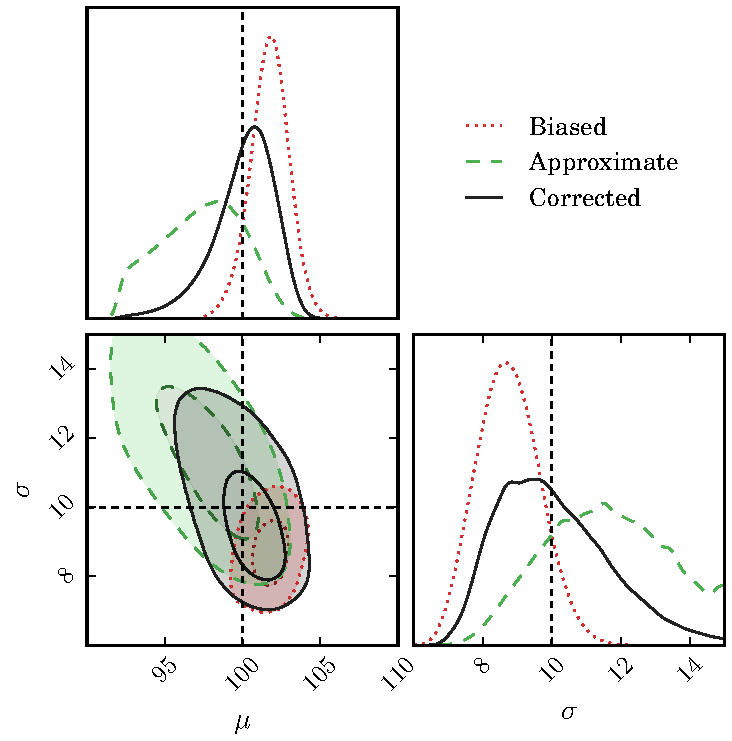
\includegraphics[width=\columnwidth]{example/real.pdf}
	\end{center}
	\caption{A systematic test of our more complicated model, done by stacking the output chains from fitting 100 independent realisations of our 100 data points, subject to our thresholding. The likelihood $\mathcal{L}_1$ was evaluated, and reweighted using Monte Carlo integration of a hundred thousand possible events as per $\mathcal{L}_2$. The truncated data with no correction is shown as `Biased' in dotted red, the `Approximate` only correction ($\mathcal{L}_1$) shown in dashed green, and the final reweighted chain shown in solid black as `Corrected'.}
	\label{fig:real}
\end{figure}















\section{Numerical Tricks}
\label{sec:tricks}

\subsection{Importance Sampling}
Further tricks can be used to increase the efficiency with which the samples are reweighted. Firstly, the overarching analytic model often provides functions which can be drawn from efficiently. In the case of our example, by drawing the random numbers $X$ and $Y$ respectively from the normal distributions $\mathcal{N}(\mu,\sigma)$ and $\mathcal{N}(\mu_y,\sigma_y)$ (ie traditional importance sampling) we need only evaluate the step function for our data points. That is, we replace
\begin{align}
\int f(X) \mathcal{N}(X|\mu,\sigma)\, dX = \frac{1}{N} \sum_{i=1}^N f(X_i) \mathcal{N}(X_i | \mu, \sigma),
\end{align}
where $X$ is drawn from a uniform distribution over all space, with 
\begin{align}
\int f(X) \mathcal{N}(X|\mu,\sigma)\, dX = \frac{1}{N} \sum_{i=1}^N f(X_i),
\end{align}
where $X$ drawn from $\mathcal{N}(X_i | \mu, \sigma)$.

\subsection{Precomputing selection}
If evaluating the probability that an event is observed is numerically expensive (i.e. not a step function), it is easy to pregenerate a set of events and reuse them for all weights - provided that the number of events used when calculating the weights is sufficient to make the statistical error of Monte Carlo integration insignificant when compared to the constraining power of your dataset. This method is however only efficient when prior knowledge of parameter values is known to allow a reasonable initial draw of events. Without this prior information, samples need to span the entire posterior volume, which is numerically intractable even for low dimensional models. 

Consider the imperfect example - where we observe $x$ drawn from an underlying normal distribution, but utilise the Monte Carlo integration technique from Section \ref{sec:real} and do not have an analytic approximation (i.e. we set $w_{\rm approx} =1$). We could estimate, given some prior knowledge, that variable $x \approx \mathcal{N}(\mu_{\rm guess}, \sigma_{\rm guess})$. We then drawn samples of $x$ from this distribution, recording the probability of each draw and then calculating whether our potential observation of $x$ would be observed in the experiment or not. That is, we assign $P(S|x,\theta) = P(S|x) = 1$ or $0$ given it passed cuts or not. We discard all events with $0$ weight (as they have $0$ weight), and only track those events which pass. Then, when calculating the sample reweighting after running chains, $\mathcal{L}_{i2}$ becomes
\begin{align}
\mathcal{L}_{i2} \propto w_{\rm approx}  \left[\sum_{j=1}^{n} \frac{\mathcal{N}(X_j | \mu, \sigma)}{\mathcal{N}(X_j | \mu_{\rm guess}, \sigma_{\rm guess})} \right]^{-1},
\end{align} 
where you can see that we discard the constant $n$ from equation \eqref{eq:mc} as we only care about likelihood proportionality. Provided our parameter estimate is reasonably well informed, the computation benefit this precomputation provides is enormous for any nontrivial selection function. Not only do we now waste no time when calculating $\mathcal{L}_{i2}$ determining $P(S|{\rm data}, \theta)$, as we only save results that pass the cuts, we have no wasted evaluations of $\mathcal{N}(X_j | \mu, \sigma)$.

The astute reader may have picked up on one assumption - that selection efficiency of an observation is independent of model parameters $\theta$. For many experimental cases this should hold, however if it does not this method cannot be used to increase efficiency. Gridding or interpolating the parameter space is strongly not recommended due the required accuracy of $\mathcal{L}_{i2}$. Even a small error when raised to the power of $N$ can spiral out of control.

\subsection{Log-space}

Following from the previous section, as our reweighting $\mathcal{L}_2$ is raised to the power of the number of our observations, they should definitely be computed in log-space, which turns the power into a linear factor. As most probabilistic work is already computed in log-space, this subsection barely needs to be stated. However, whilst working in log-space an efficient way of increasing the accuracy of the approximate analytic correction is to fit the correction such that the spread of the distribution $\log\mathcal{L}_2$ is minimised. 














\section{Conclusion}
\label{sec:conclusion}


Sample selection is a pervasive issue in many scientific domains. For simple cases of sample selection which can be encapsulated with analytic functions, it is possible to analytically correct likelihood surfaces by introducing selection efficiency into the likelihood formulation. When analytic corrections fail to provide an adequate description of selection effects, Monte Carlo integration can be used on top of analytic approximations to further correct the likelihood surface, provided the experiment can be effectively simulated. 



\section*{Acknowledgments}

We gratefully acknowledge the input of the many researchers that were consulted during the creation of this paper.

\bibliography{bibliography}

% Don't change these lines
\bsp	% typesetting comment
\label{lastpage}
\end{document}

% End of mnras_template.tex

